\subsection{Use Case}

\subsubsection{User Registration}

	% example \usecase{name}{actor}{goal}{precondition}{post condition}{flow}{exception}


	
	
	
	\usecase{User Registration}
				{Guest}
				{\goal{1}}
				{Guest hasn't registered to the webapp yet.}
				{Guest is signed-up and promoted to ``PowerEnJoy'' User.}
				{
					\begin{enumerate}
						\item Guest accesses to the webapp or the mobile application
						\item Guest clicks on ``Sign Up'' button
						\item Guest fill Sign-up form fields, entering\\
						-Name\\
						-Surname\\
						-Email address\\
						-Password\\
						-Telephone Number\\
						-Driving License number
						\item Guest accepts the term of use
						\item Guest clicks on ``Confirm'' button\end{enumerate}
				}
				{-}
				{
				\begin{enumerate}
					\item At least one field is empty
					\item At least one field is invalid
					\item Entered email is already associated to another account\end{enumerate}
				}
	



\pagebreak
\subsubsection{User Login}

\usecase{User Login}
{User}
{\goal{2}}
{User has signed-up as PowerEnJoy User.}
{User is redirected to personal area.}
{
	\begin{enumerate}
		\item User accesses to the webapp or the mobile application
		\item User clicks on ``Log-in' button
		\item User fills username and password fields of Log-in form
		\item User clicks on ``Submit'' button
	\end{enumerate}
}
{-}
{
	\begin{enumerate}
		\item Invalid username and/or password
		\item At least one field is empty
	\end{enumerate}
}

\begin{figure}[h]

	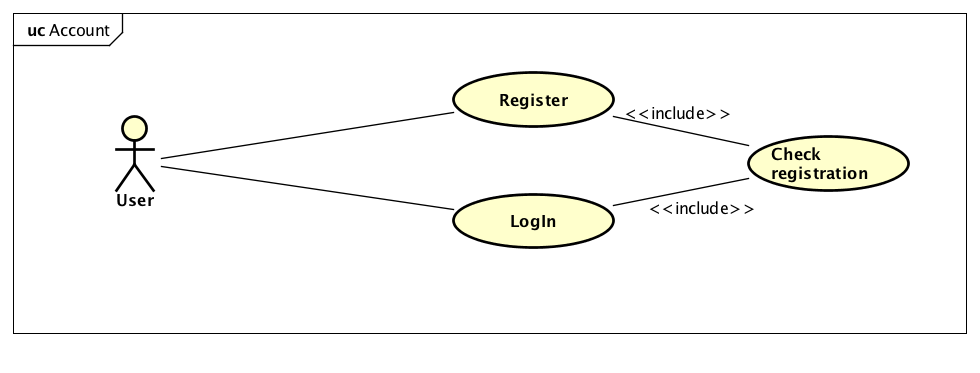
\includegraphics[width=380px]{img/usecase_login_registration}
	\caption{Use Case Login and Registration procedure. Refer to Goal 1 and 2}
\end{figure}

\newpage


\subsubsection{Modification of personal details and payment information}


\usecase{Modification of personal details and payment information}
{User}
{\goal{3}}
{User is logged in}
{User is redirected to the modifications area where he can modify his personal information}
{
\begin{enumerate}
	\item User accesses to the webapp or the mobile application
	\item User logs in
	\item User clicks on ``Personal Details'. A page with the personal data of the user is shown'
	\item User clicks on ``Modify Data'' button. A form for modifications is shown
	\item User fills fields he wants to modify
	\item User clicks on ``Confirm'' button
	\item User is redirected to his personal area
\end{enumerate}
}
{-}
{-}


\newpage
\subsubsection{Search of available cars}\label{search}

\usecase{Search of available cars}
{User}
{\goal{4}}
{User is logged in}
{User is redirected to a page with the list of the available cars}
{
\begin{enumerate}
	\item User accesses to the webapp or the mobile application
	\item User logs in
	\item User clicks on ``Search a car'' button. A form is shown
	\item User select a distance from the ``Distance from your position'' field
	\item User clicks on ``Confirm'' button
	\item User is redirected to a page showing the available cars
\end{enumerate}
}
{
\begin{itemize}
\item Different flow from step 4:
	\begin{enumerate}
	\item[4] User write an address in the ``Address'' field 
	\item[5] User clicks on ``Confirm'' button
	\item[6] User is redirected to a page showing the available cars
 
\end{enumerate}

\end{itemize}


}
{
\begin{enumerate}
\item There aren't available cars within the distance set 
\item There aren't available cars near the address set
\end{enumerate}
}

\subsubsection{Search of resources on a map}\label{search2}

\usecase{Search of resources on a map}
{User}
{\goal{5}}
{User is logged in}
{User is redirected to a page with a map where resources (available cars, safe areas, special parking areas)  are shown}
{
\begin{enumerate}
	\item User accesses to the webapp or the mobile application
	\item User logs in
	\item User clicks on ``Search resources on the map'' button. A form is shown
	\item User select a distance from the ``Distance from your position'' field
	\item User clicks on ``Confirm'' button
	\item User is redirected to a page showing the resources on a map.
\end{enumerate}
}
{
\begin{itemize}
\item Different flow from step 4:
	\begin{enumerate}
	\item[4] User write an address in the ``Address'' field 
	\item[5] User clicks on ``Confirm'' button	
	\item[6] User is redirected to a page showing the resources on a map.
 
\end{enumerate}

\end{itemize}


}
{
\begin{enumerate}
\item There aren't available cars within the distance set 
\item There aren't available cars near the address set
\end{enumerate}

}

\subsubsection{Request}

\usecase{Request}
{User}
{\goal{6}}
{User is logged in}
{The car requested is reserved for the user}
{
\begin{enumerate}
	\item User accesses to the webapp or the mobile application
	\item User logs in
	\item User searches a car (use case ~\ref{search})
	\item User select a car from the list. 
	\item A page with information about the car (battery level, model) is shown
	\item User clicks the ``Request'' Button''
	\item The car is reserved for the user
\end{enumerate}
}
{
\begin{itemize}
\item Steps 3 and 4 are different:
	\begin{enumerate}
	\item[3] User searches a car (use case ~\ref{search2})
	\item[4] User select a car on the map.   
	\end{enumerate}

\end{itemize}


}
{
\begin{enumerate}
\item The car selected has been requested by another user before the User has clicked on the ``Request'' button.
\end{enumerate}

}


\FloatBarrier


